% Created 2019-11-12 Tue 16:27
% Intended LaTeX compiler: pdflatex
\documentclass{article}
\usepackage[utf8]{inputenc}
\usepackage[T1]{fontenc}
\usepackage{graphicx}
\usepackage{grffile}
\usepackage{longtable}
\usepackage{wrapfig}
\usepackage{rotating}
\usepackage[normalem]{ulem}
\usepackage{amsmath}
\usepackage{textcomp}
\usepackage{amssymb}
\usepackage{capt-of}
\usepackage{hyperref}
\usepackage{times}
\author{Britt Anderson}
\date{\textit{<2019-04-30 Tue>}}
\title{Introduction to Computing for Psychology Students}
\hypersetup{
 pdfauthor={Britt Anderson},
 pdftitle={Introduction to Computing for Psychology Students},
 pdfkeywords={},
 pdfsubject={Add description of the program here! And Review section},
 pdfcreator={Emacs 26.2 (Org mode 9.2.3)}, 
 pdflang={English}}
\begin{document}

\maketitle
\tableofcontents

\section{Course Goal:}
\label{sec:orgd2ffb55}
Improve your ability to use your computer as a tool for academic activities.

This leads to the following learning objectives
\section{Learning Objectives:}
\label{sec:orgc979218}
\begin{itemize}
\item Learn how to install software.
\item Learn how to work from the command line.
\item Learn the rudiments of programming sufficient to allow further progress through self study.
\item Learn about the use of libraries to enable programming psychological experiments.
\item Learn how to use version control
\item Learn how to write papers that blend code and analyses to generate reproducible research reports.      
This includes learning
\begin{itemize}
\item how to use citation databases
\item generate graphics of analyses
\item conduct statistical analyses
\item generate multiple output formats from a single source file.
\end{itemize}
\end{itemize}
\section{Course Mechanics}
\label{sec:org047374d}
To meet the learning objectives you will need to \textbf{do} more than you listen or observe. You will also need to break old habits. That means in the beginning it will be harder to do simple things. It also means that in the future things that used to be impossible for you to do will now be possible (but they may still not be easy). Combining computer skills with with your psychology content knowledge makes you more attractive to employers and on a graduate school application. 

Thus, this course will require you to use the Linux operating system (the XUbuntu flavor) and tools available within that space. Later on, after this course, if you wish to return to the world of OSX and Windows10 you will know what you are looking for, and you will have the skills necessary to make it available. 
\section{Outline}
\label{sec:org5c18a90}
\subsection{Session 1 Installing Linux}
\label{sec:orged7cf70}
\subsubsection{Instructions for testing the Live CD and installing to USB}
\label{sec:orge3426ae}
\begin{enumerate}
\item Learn how to boot your computer from a USB. 
\begin{itemize}
\item Mac OSX - start the computer with option key held down
\item Windows - may require going into the bios and enable booting usb (usually some key combo of F2 or F10 during the boot process - look for a very briefly flashed screen); followed by rebooting with a different F Key. Another option is to tell Windows to boot from recovery mode. Find the "advanced" menu of the Windows Start Up menu (look in the "recovery" section of the start-up). Select from "another device". Some devices, like Surfaces, have other key combinations.
\item Other systems: chrome books; ipads; probably won't work.
\item Sometimes it takes a while to figure out which of the options is the Xubuntu option. If one doesn't work, just note what it was and next time try a different one.
\end{itemize}
\item Run an XUbuntu Live CD (off us USB)
If problems starting the use without installing option, restart, select install, and then quit from the first screen. That will usually drop you into what you need.
\item Make sure to set the screen off and power off power management features to "never". This can hurt you if you are waiting on a download and the computer goes to sleep. It may not wake normally, and it can damage the USB.
\item Explore the Live USB
\begin{enumerate}
\item Connect to the wifi.
\begin{enumerate}
\item Click up/down arrow in upper right corner of the screen.
\item Select the correct options (to be demonstrated).
\begin{itemize}
\item Authentication: PEAP
\item Click box no certificate required
\item Use your full watiam address (including the stuff after @ sign usually).
\end{itemize}
\end{enumerate}
\item Verify working by opening Firefox Web Browser
\begin{enumerate}
\item Click little icon upper left.
\item From the dropdown menu select \emph{Web Browser}.
\item Go to \url{https://uwaterloo.ca}
\end{enumerate}
\item Explore some of the other programs available in the dropdown menu and under the different headings.
\begin{enumerate}
\item Which program is like Word for Windows?
\item How do you take a screenshot?
\item What is the standard email program on this version of Linux?
\end{enumerate}
\item Installing programs
There is a "gui" installer, but we are going to use the package management system from the command line.
\begin{enumerate}
\item Open the terminal emulator
\item type \texttt{sudo apt update}
What does \emph{sudo} mean?
\item Do \textbf{NOT} upgrade your old packages at this point.
\item type \texttt{sudo apt install emacs} ; accept the defaults
\item Leave the terminal open but drag over to the menu in the upper left corner and inspect the \emph{Development} folder. You should emacs in there. Do \textbf{not} click it. We are going to launch from the command line.
\item Back in terminal type: \texttt{emacs \&}.
What does the ampersand do? It lets things run in the background without freezing the terminal. If you don't know what I mean, then start without the ampersand, and then try to type another command in the terminal. Remember: if you don't know what will happen? Try it (after maybe backing up important files).
\item Go to the emacs help menu and under the drop down options pick emacs psychotherapist. Remember it is here when you need some counselling in the first few sessions of this course.
\end{enumerate}
\end{enumerate}
\item Syllabus review (short break).
\item Problems with the live "CD". 
Nothing is permanent. All your upgrades and installations vanish everytime you turn it off and you would have to do it all over again everytime you restart. So, I want you to install Xubuntu so that any changes you make will be persistent, but since I don't want to require you to alter your personnel machine, will will install it to a usb and you will then run your computer from this new, second, usb where the changes you make will persist.
\item Install Linux XUbuntu to a second USB
This will be the major goal of the rest of our session. Follow the prompts on the screen. Work together. Ask questions. 

\textbf{\textbf{Where you need to be careful}}

When you install software you need to make sure that install it to the usb and not the hard drive on the computer. Also, beware the boot loader. This is the program that helps your computer start and chooses an operating system. If you install it in the wrong place you may not be able to boot your Xubuntu installation or you may need the live disc to boot your non-linux installation. If you go slow and are careful the risk of either of these events is small. 

Note: Don't choose to small a USB. 8GB will work to install the base system just fine, but when you try to add further software you will fill up the disc quickly and then you will have to start all over. 16GB should work, but 32 GB is a safer choice if you imagine downloading a lot of s
For more detailed instructions go to the section \hyperref[sec:orgc5688be]{Instructions for Burning Xubuntu to a USB}
\item When you think you are done, shut things down. Remove the live USB/CD, but leave the other one in place. Follow the steps you need to to boot your computer from a USB. If you are able to launch Ubuntu (and it might take a few tries to find the right menu entry) then you will see linux start. Enjoy the feeling of immense power.
\item Boot your computer from the \emph{new} USB and install \textbf{emacs} \emph{from the command line} again.
\begin{enumerate}
\item The command line - open up a "terminal". Your terminal will be running a "shell."
\item Package Managers
\begin{enumerate}
\item The ubuntu package manager
Basic commands: 
\begin{itemize}
\item apt update
\item apt install
\item apt search
\item apt remove
\end{itemize}
\end{enumerate}
\end{enumerate}
\item This time you might want to update those old programs.
\end{enumerate}
\subsubsection{Troubleshooting}
\label{sec:orgba353b3}
\begin{description}
\item[{I don't have a USB port?}] Do you have an sdcard port? Yes? You can use that. If you have neither you will need a different computer. It can be a cheap (as in the price of textbook cheap) and old one.
\item[{I only have one USB port.}] Can you work with a neighbor to repeat the installation instructions on a second USB that you can use on your machine? If not, you may need something like this. 
\url{https://images-na.ssl-images-amazon.com/images/I/81j1TYALbYL.\_SL1500\_.jpg}
\item[{Can I just install Linux on my computer?}] You certainly can, and you can even keep you "old" operating system and use one or the other as you choose. But this seemed more than I could require of all students, but I encourage you to do it if you are willing. First, \textbf{\textbf{back up everything}} because trying this and getting it wrong could cause you to lose all your saved information.
\item[{I already use Linux.}] Good for you. Help a classmate.
\item[{What is Linux?}] Check wikipedia.
\item[{Why use Xubuntu?}] Is it different from Ubuntu (Debian, Arch, Fedora, OpenSuse\ldots{})? Linux is a kernel that powers the system. All the rest are different choices people make of the tools they want to wrap around that "engine." XUbuntu is a reasonably light-weight linux distribution that runs well on slow machines, and yet has enough of a user base to make it reasonably easy to find help on line.
\end{description}
\subsubsection{Homework}
\label{sec:org6832871}
\begin{enumerate}
\item Send me a screenshot of emacs open and running on your laptop.
Hints: look for xfce4-screenshooter to take the screenshot. Log on to \emph{Learn} while running linux. Of course that will require you to connect to the internet, and that will require you repeating those steps to configure the connection.
\item Look at the available software applications and download one (1). Don't go crazy on this. You are running your whole computer from a small usb, it will already be slow, and you will already be limited for space. Just find one program (look for "software" in the upper left corner icon drop down menu) that strikes you as cool or interesting and install it, play with it, and write a one-paragraph description of it using this format:

\begin{verbatim}
* Package Name
  My Package
** Short Description
   A package for something.
** Review
   I liked it because ... and so on.
\end{verbatim}

Save it with yourlastname-firstname\(_{\text{pkgname.org}}\) as the file name. Upload it to the dropbox on learn. And save it, because you will need it again soon. 

Use the program "mousepad" for the above.
\end{enumerate}
\subsection{Session 2 Command Line Basics and EMACS Introduction}
\label{sec:org373872b}
\subsubsection{Command Line}
\label{sec:orgdb7e987}
\begin{enumerate}
\item What is it?
\label{sec:org279b5cb}
\item Why use it? \href{https://www.quora.com/How-important-is-it-to-learn-command-line-interfaces/answers/1620528}{One opinion.}
\label{sec:org103b708}
\begin{enumerate}
\item The \href{http://write.flossmanuals.net/command-line/introduction/}{Manual}
\label{sec:orgfb985ac}
\end{enumerate}
\item Find your terminal?
\label{sec:org02c4cc9}
Why is it called the terminal?
\begin{enumerate}
\item Operating Systems
\label{sec:org646bde1}
\begin{itemize}
\item Windows
\begin{itemize}
\item \href{https://www.howtogeek.com/235101/10-ways-to-open-the-command-prompt-in-windows-10/}{CMD}
\item \href{https://docs.microsoft.com/en-us/powershell/scripting/getting-started/getting-started-with-windows-powershell?view=powershell-6}{Power Shell}
\item \href{https://docs.microsoft.com/en-us/windows/wsl/install-win10}{WSL} 
If you use this I recommend you install the Ubuntu version. That is
the one that I know the most about from the options. Note that
this will give you access to command line tools, but not to
graphical tools.
\item \textbf{\textbf{Recommended}} If you have windows 10 you can run linux as a
\href{https://www.windowscentral.com/how-run-linux-distros-windows-10-using-hyper-v}{virtual machine}.
\end{itemize}
\item OSX
\begin{itemize}
\item Applications/Utilities/Terminal
\item Why don't you have to install a virtual machine to get linux commands on OSX?
\end{itemize}
\item Linux 
\begin{itemize}
\item probably xterm
\end{itemize}
\end{itemize}
\end{enumerate}
\item Terminal Games
\label{sec:orgd7cba41}
\begin{enumerate}
\item \texttt{ls -la /home/<username>}
\begin{itemize}
\item What does all this output mean?
\item What changes when you leave out the \texttt{-la}?
\item What does the hyphen do?
\end{itemize}
\item Find the location of your Desktop folder.
\item Change to that directory.
\texttt{cd}
\item Find out where you are?
\texttt{pwd}
\item Find out how much free space you have on your computer disk.
\texttt{df -h}
\item How do you get help for most of these commands?
Usually \texttt{command -{}-help} or (\texttt{-h})
\item How do you find the manual?
\texttt{man ls}
\item Navigating
\begin{enumerate}
\item Paths: absolute and relative.
\item What do those "dots" mean?
\item What do those slashes mean?
\item Tab is your friend.
\item Try the up arrow too.
\end{enumerate}
\item File ownership
\begin{enumerate}
\item Make a text file from the command line.
\texttt{touch /home/yourname/Documents/testText.txt}
\item Who owns it?
\end{enumerate}
\item Make a directory
\texttt{mkdir /home/britt/Documents/myFirstDir/}

Spaces are the enemy. Never use them, but if you have to, escape (\texttt{\textbackslash{}}) them.
\item Want more practice? Try the tutorials \href{https://ryanstutorials.net/linuxtutorial/commandline.php}{here}.
\end{enumerate}
\end{enumerate}
\subsubsection{Exercises Emacs}
\label{sec:org3173899}
\begin{enumerate}
\item Emacs
\label{sec:orgfabaa88}
\begin{enumerate}
\item What are Control and Meta used for? What keys are they?
May depend on your keyboard and operating system. Don't like what they are? \href{https://www.x.org/releases/current/doc/man/man1/xmodmap.1.xhtml}{Remap them}.
\item Tutorial \texttt{Ctrl-h t} (aka \texttt{C-h t})
\item Find the Psychotherapist - you may need it.
\item Play a game - try \texttt{M-x tetris}
\item Init files and packages. 
Emacs has it's own package system that allows you to greatly expand its functionality. Most of those customization are set up in your \texttt{\textasciitilde{}/.emacs.d/init.el} file. Create it if it doesn't exist. 

You can learn more by reading the \href{emacs\#Init\%20File}{info file}.

A minimal init.el to get started. And make sure your emacs package is update to the latest version. 

This can be a bit tricky to get started because you will have to first install \texttt{use-package} manually via \texttt{package-list-packages} where you mark it with an \texttt{I} and the \texttt{x}. Then close and restart emacs.  From here on out you can add the packages to your init where you customize them and then they get downloaded as needed. 

\begin{verbatim}
(require 'package)
(add-to-list 'package-archives '("melpa" ."http://melpa.org/packages/") t)
(package-initialize)


(use-package elpy
   :ensure t
   :init (elpy-enable))

(use-package ess
  :ensure t
  )
\end{verbatim}

If you get errors about gnupg and signing signatures.

You can try this code to make sure that gnupg has the directories established that it needs and has "signed" the correct security key for emacs packages. 

\texttt{gpg -{}-homedir /home/<NAMEOFYOURHOMEDIRHERE>/.emacs.d/elpa/gnupg  -{}-keyserver keyserver.ubuntu.com -{}-recv-keys 066DAFCB81E42C40}
\end{enumerate}


\begin{enumerate}
\item Program your editor
\begin{enumerate}
\item Turn off the tool bar?
\item How? \texttt{C-h-f} will allow you to search for functions. Try the keyword menu and tab and see if you come across a likely contender (\texttt{menu-bar-showhide-tool-bar-menu-customize-disable}).
\item Navigate to the scratch buffer. Put that function in parantheses. Move to the end. Type \texttt{C-x C-e}. Did your tool bar go away?
\item Point is that you can heavily customize your editor. Don't worry too much about it for now.
\end{enumerate}
\item \href{org\#Top}{Orgmode}
\begin{enumerate}
\item What is it? About the best thing ever.
\item Make an outline. Keep a calendar. Add code to your documents. Make links. Include images.
\item Practice now:
Where is the help, remember? \texttt{C-h i}
Note bene: may need to get \texttt{sudo apt install emacs25-common-non-dfsg} for all the documentation. 
\begin{enumerate}
\item Learn to use the short cuts to open, save, and so on. That is one of the powers of the command line and similar style tools. Enhance your productivity and control.
\item Create an outline.
\item Create a link
\item Insert an image
\item Export as a web page.
\item What would you need to export a pdf?
Try installing \texttt{texlive-latex-base texlive-latex-extra}. If that doesn't work, repeat with \texttt{texlive-latex-recommended}. If that doesn't fix the problem go with \texttt{texlive-full}. This is big. Be patient.
\end{enumerate}
\end{enumerate}
\end{enumerate}
\end{enumerate}
\subsection{Session 3 Version Control Github and Beginning With Python}
\label{sec:org3c89647}
\subsubsection{Version Control}
\label{sec:org325e6c6}
\begin{enumerate}
\item Git
\label{sec:orgd15c8e0}
\textbf{\textbf{Not}} the same as Github, though that is one of the more common \emph{social} uses of git for sharing and collaborating on code. 
\item Social Coding and Data Sharing
\label{sec:orgf7c6d0f}
A brief discussion of what is going on here.
\begin{enumerate}
\item OSF.io
\label{sec:org1cd5446}
\begin{enumerate}
\item Sign up
\item Find my projects
\end{enumerate}
\end{enumerate}
\item Installation of Git
\label{sec:orgdc16590}
\texttt{sudo apt install git}
\item Github and Gitlab and Bitbucket and \ldots{}
\label{sec:org5f36a6d}
\begin{enumerate}
\item Github is the big one with a large external presence.
\begin{enumerate}
\item Sign-up
\end{enumerate}
\item The university provides you with a gitlab presence at \url{https://git.uwaterloo.ca}
\end{enumerate}
\item Git
\label{sec:org87f076a}
\begin{enumerate}
\item Open a terminal
\item Move (\texttt{cd} or \texttt{dir}) into your Desktop
\item type \texttt{git init myrepo}
\item Should see message from the terminal prompt that it has been created.
\item Feel free to delete (e.g. \texttt{rm -rf ./myrepo})
\end{enumerate}
\item Making and Cloning a Course Repo
\label{sec:org16143cd}
\begin{enumerate}
\item I create an empty repository on github
\item I create a repository on my laptop.
\item I add some small file.
\item I set the upstream (origin) as the github site, and then I push.
\item Now if I use a different computer I can push and pull (to be discussed) from this github site and keep everything synced together.
\end{enumerate}
\item Demo the Course Git Site
\label{sec:org3bd26f6}
I am keeping back-ups of my notes for this course on github. You can get everything I create by cloning this repository.
\begin{enumerate}
\item Go to \href{https://github.com/brittAnderson/psych363}{Course Repo on Github}
\item Use that url to clone a copy to your laptop (or to fork a version to your github account). Occassionally \texttt{pull} in any changes or updates.
\item You will probably find it easier to skip the fork step for any repository that you are just going to use, but not change.
\end{enumerate}
\item Magit
\label{sec:orgb8c4a41}
\begin{enumerate}
\item Emacs provides you with an interface for this called magit.
\item To use it you will have to create an init file (and delete \textasciitilde{}/.emacs)
Let's you discover the hidden directories.
\item You will have to enable emacs package repositories (everyone in linux land has a package manager).
\item You will need to install the magit package.
\item Then it is \texttt{C-c m} or \texttt{M-x magit}
\end{enumerate}
\item Forks and Clones and Pull Requests\hfill{}\textsc{homework}
\label{sec:orgcf1189e}
\begin{enumerate}
\item Diagram the logic on the board.
\item Get everyone to create a fork of the course repository
\item Get everyone to create a local clone on their laptop
\item Set a second upstream pointing to me.
\item Pull from my repo to laptop.
\item Update and accept the changes.
\item Push this to your fork.
\item Add a new file to your laptop version.
\item Push this to your fork.
\item From github generate a pull request for me. This is one of this weeks homeworks.
\end{enumerate}
\end{enumerate}
\subsubsection{Beginning Python}
\label{sec:orga64a2cf}
\begin{enumerate}
\item Python
\label{sec:org6356bb9}
\begin{enumerate}
\item Test for Python in a terminal.
\begin{itemize}
\item open a terminal
\item type \texttt{python -{}-version} then \texttt{enter}
\item If you see an answer you have python. Type \texttt{python}. Note the cursor has changed.
\item type \texttt{2 + 2 enter}
\item Do you see 4?
\item type \texttt{quit()} to exit.
\item Why do you need to have the parentheses after the word quit?
\end{itemize}
\item If you only have version 2 try the command again with \texttt{python3 -{}-version}.
\item If you don't have python3, get it (may want the python3-dev version; often the hyphen -dev packages will work better for you as a bleeding edge user).
\end{enumerate}
\item Coding - General
\label{sec:org68af42f}
Coding - providing instructions to a computer.
The computer only does what you tell it. 
\item Writing Code
\label{sec:orgd1182ad}
Code files are just plain text. You can open and write them in anything, though some tools can make the writing substantially easier. Usually extensions identify a language (e.g. .py for python and .R for R). 
\item Testing Code
\label{sec:orgb060ce4}
\begin{enumerate}
\item Interactive
\label{sec:org5f41e56}
We already did a little of this, but let's try again.

\begin{verbatim}
def myadd(a,b):
    return(a+b)
\end{verbatim}

\begin{verbatim}
print(myadd(3,4))
\end{verbatim}

\begin{verbatim}
Traceback (most recent call last):
  File "<stdin>", line 1, in <module>
NameError: name 'myadd' is not defined
\end{verbatim}

For interactive session it is like you are interacting with a user. You type your lines one or a few at a time, get an answer, and then decide what to do next. 
\item Script
\label{sec:org5dd35dc}
You write a separate file that you read in, or import and use. Here is the file.

def add2(a,b):
    return(a+b)

def addMany(aa):
    ans = 0
    for a in aa:
	ans = ans + a
    return(ans)

\begin{verbatim}
from code.testScript import *

print(add2(3,4))

print(addMany([1,2,3,4,5,6]))
\end{verbatim}

\begin{verbatim}
7
21
\end{verbatim}

Try creating this file and then typing these commands in your terminal. For various weird reasons if you want the test script to be in a subdirectory of where you are working you will need a file \texttt{\_\_init\_\_.py} to trick python into treating it as a package. See the \href{https://docs.python.org/3/tutorial/modules.html\#packages}{documentation} and this \href{https://stackoverflow.com/questions/1260792/import-a-file-from-a-subdirectory}{stackOverflow answer}.
\end{enumerate}
\item Confirming You Can Write and Run a Python File\hfill{}\textsc{homework}
\label{sec:orgcd19c89}
\begin{enumerate}
\item Create a file \texttt{lastname.py}
\item Write the myadd function I demonstrated, but give it a different name.
\item Save.
\item Open up a terminal.
\item Start a python session.
\item Import your file with you function.
\item Use your function.
\item Take a screenshot of your terminal session showing the above session.
\item Submit that for your homework \textbf{along with your lastname.py file}.
\end{enumerate}
\end{enumerate}
\subsection{Session 4 Python}
\label{sec:org6e744b7}
\subsubsection{Types}
\label{sec:orgd9e97b9}
\begin{description}
\item[{Integers}] 1, 2, \ldots{}
\item[{Doubles/Floats}] 10.3, pi
\item[{Booleans}] True , False 
NB: some languages, e.g. R, use TRUE.
\item Lists and Tuples
\begin{description}
\item[{Tuples}] (1,2), ('a',10.34,False) Have a fixed number of slots, can be different types.
Define with parentheses
\item[{Lists }] [1,2,3,4] Have a potentially infinite number of slots, but must all be same type.
Define with square brackets.
\end{description}
\item[{Dictionaries}] \{'firstName' : 'Britt', 'lastName' : 'Anderson'\}
\item[{Comments}] Not really code, but allows you to put stuff in your programs for other users and yourself to read. In python the lines start with a hash "\#"
\end{description}
\subsubsection{Constants and Variables}
\label{sec:orgb0a091b}
A conceptual difference more than a implementation difference
\begin{verbatim}
NOHRSDAY = 24

x = NOHRSDAY

x
\end{verbatim}

\begin{verbatim}
24
\end{verbatim}

\begin{enumerate}
\item Coding styles
\label{sec:org1d127f7}
Makes your code easier to read by people using the same language.

Try to follow good programming style, and if avaialable, langugage guides.

\href{https://www.python.org/dev/peps/pep-0008/}{Python Style Guide}
\end{enumerate}
\subsubsection{Assignment and Equality}
\label{sec:org945a716}
\texttt{=} is different from \texttt{==}

\begin{verbatim}
a = 2
print(a == 3)
\end{verbatim}

\begin{verbatim}
False
\end{verbatim}

\subsubsection{Loops}
\label{sec:orgce8d366}
Think of recipes: "stir egg whites until peaked" or "simmer for 30 minutes". That is the intuition for a 
\begin{enumerate}
\item For
\label{sec:orgd1324e8}
Python refers to things called "iterables." To iterate is another way of saying something you can keep doing the same thing over and over to. Imagine a bowl of ice cream. It is "eatable". You take one spoon, and keep taking spoonfuls until the bowl is empty. 
\begin{enumerate}
\item Indexing
\label{sec:orgb1e546b}
You can get the location of an element in a list by referring to its \emph{index}. Indexes start at 0 for many computer languages, but not all (e.g. R and Matlab). There are various shorthands for getting ranges of elements or the last element.

\begin{verbatim}
nameDict = {'firstName' : 'Britt', 'lastName' : 'Anderson'}
mylist = list(range(1,10))

print(nameDict['firstName'])

print(mylist)

print(mylist[0])

print(mylist[-1])

print(mylist[0:4])
\end{verbatim}

\begin{verbatim}
Britt
[1, 2, 3, 4, 5, 6, 7, 8, 9]
1
9
[1, 2, 3, 4]
\end{verbatim}


\begin{verbatim}
for ml in mylist:
    print(ml)


for i,ml in enumerate(mylist):
    print("The {0}th element was {1}".format(i,ml))
\end{verbatim}

\begin{verbatim}
1
2
3
4
5
6
7
8
9
The 0th element was 1
The 1th element was 2
The 2th element was 3
The 3th element was 4
The 4th element was 5
The 5th element was 6
The 6th element was 7
The 7th element was 8
The 8th element was 9
\end{verbatim}
\item For Class Exercise
\label{sec:org2218da4}
\begin{enumerate}
\item Create a list of at least 8 individual characters.
\item Make sure they are \textbf{\textbf{not}} in alphabetical order
\item Print the letters one at a time.
\item Print the letters sorted alphabetically one at a time, but \emph{do not} overwrite your original list.
\item Print the letters from both lists with a format command that says which position the letter is in.
\end{enumerate}

\begin{verbatim}
myList = list("brittAnderson")
for l in myList:
    print(l)
print("end of list 1\n")


for l in sorted(myList):
    print(l)
print("end of list 2\n")


for i,l in enumerate(zip(myList,sorted(myList))):
    print("The {0}th letter of myList is: {1}, but is {2} in the sorted list.".format(i,l[0],l[1]))
print("Thus ends the lesson")
\end{verbatim}

\begin{verbatim}
b
r
i
t
t
A
n
d
e
r
s
o
n
end of list 1

A
b
d
e
i
n
n
o
r
r
s
t
t
end of list 2

The 0th letter of myList is: b, but is A in the sorted list.
The 1th letter of myList is: r, but is b in the sorted list.
The 2th letter of myList is: i, but is d in the sorted list.
The 3th letter of myList is: t, but is e in the sorted list.
The 4th letter of myList is: t, but is i in the sorted list.
The 5th letter of myList is: A, but is n in the sorted list.
The 6th letter of myList is: n, but is n in the sorted list.
The 7th letter of myList is: d, but is o in the sorted list.
The 8th letter of myList is: e, but is r in the sorted list.
The 9th letter of myList is: r, but is r in the sorted list.
The 10th letter of myList is: s, but is s in the sorted list.
The 11th letter of myList is: o, but is t in the sorted list.
The 12th letter of myList is: n, but is t in the sorted list.
Thus ends the lesson
\end{verbatim}
\end{enumerate}

\item While
\label{sec:org4f0d84e}
These are like for loops in that they do stuff over and over, but unlike for loops they do things indefinitely, until that is, you tell them to stop. How do you do that? You use a predicate that they test for each time through the loop. That means you need to specify a \emph{predicate.}
\begin{enumerate}
\item Conditionals
\label{sec:org44b0cf5}
This is where you test whether something is or is not \texttt{True}. Note that Python, but not all computer languages, treats 0 as the same as False, and all non-zero values as True. 

\begin{verbatim}
if (2 == 3):
    print("Wha.....?\n\n")
elif (3 == 2):
    print("Now that is odd")
else:
    print("2 does not equal 3.")
\end{verbatim}
\item While
\label{sec:org65efaa3}
NB: note the use of colon (:) at the end of the \texttt{for} and \texttt{while} lines. 
\begin{verbatim}
i = 0
while (i<=10):
    print("brittAnderson"[i])
    i = i+1
\end{verbatim}

\begin{verbatim}
b
r
i
t
t
A
n
d
e
r
s
\end{verbatim}
\end{enumerate}
\end{enumerate}

\subsubsection{Functions}
\label{sec:org32fb45f}
You have seen an example of this before. Think of a function as a machine that grinds meat. You pour in a cow. You get out hamburger. Input. Output. Note that arguments are "local". They are not referring to variables outside, in the program globally, but only make sense locally in the function. You drop values into those slots, and they you can use those names  in your function, because until you use it, your function doesn't know what it will be getting. 
\begin{verbatim}
def myadd(x,y):
   return(x+y)
\end{verbatim}

\begin{verbatim}
myadd(2,3)
\end{verbatim}

\begin{verbatim}
5
\end{verbatim}

\begin{enumerate}
\item Class Exercise with Functions\hfill{}\textsc{homework}
\label{sec:org5b4135d}

\begin{enumerate}
\item Hangman Game
\label{sec:orga2a232c}
You will be required to turn this in, but you can get started now. 
\begin{enumerate}
\item Look up how to get user input from python on the command line.
\item Write a script that implements elements of the hangman game.
\item Your script should ask for guesses for letters in the word.
\item Give an update on the letters guessed and the missing spaces
\item Track that guesses have not exceeded max
\item Report if one or lost.
\item I will give some hints and examples in class to start us off.
\end{enumerate}
\end{enumerate}
\end{enumerate}
\subsubsection{Libraries\hfill{}\textsc{classdiscussion}}
\label{sec:org2c56b66}
Lots of people use python. If you can think that someone ought to have done \ldots{} they probably have. Use libraries whenever you can, because \ldots{} discussion points. 
\begin{enumerate}
\item What are some popular libraries?\hfill{}\textsc{classactivity:homework}
\label{sec:org44dc0c6}
\href{https://pythontips.com/2013/07/30/20-python-libraries-you-cant-live-without/}{Here} are 20 recommended ones.

Of particular note for us are:
\begin{enumerate}
\item Numpy
\item Scipy
\item Matplotlib
\item Pillow
\item Sympy
\end{enumerate}

Divide class into small groups. Assign a library. Have them present to us what it is good for, and maybe a short demo. 

Homework: Submit a short .py script to the class github repo that demonstrates the importation of your library and some basic use.
\end{enumerate}
\subsubsection{Programs}
\label{sec:orgd8a7852}
Nothing else really, but the more prolonged and complicated concatenation of the above. 
\subsubsection{Debugging and Basic Working Methods}
\label{sec:org9ca7546}
The most basic is just to \texttt{print} statements into your code so that you can see what happening and whether your variables are actually what you think they should be. 
\subsubsection{IDEs}
\label{sec:orgc21d487}
What does IDE stand for?

What are common IDEs for python and how do you get them. What are they good for. 

Two popular ones are:
\begin{enumerate}
\item Spyder
\item pyCharm
\end{enumerate}

This is what you need to use for this course: emacs.
\begin{enumerate}
\item Open up a blank file with a name that ends in .py
\item Type in some lines (e.g. a = 2, b = 3, print(a+b))
\item Type C-c C-c on the first line.
\item Read the error message
\item Fix it.
\item Keep C-c C-c'ing on each line and look at what is happening in your console.
\item When your cursor is on a python word, like \texttt{print}, look in the mode line.
\item Try M-x linum-mode
\item To see some fancier stuff install the \texttt{elpy} package for emacs.
\begin{enumerate}
\item M-x package-list-packages
\item C-s elpy
\item type "i"
\item type "x"
\end{enumerate}
\item An easier way to get and maintain your emacs package is "use-package". See some instructions \href{https://elpy.readthedocs.io/en/latest/introduction.html\#overview}{here}.
\item When you try \texttt{(elpy-enable)} you will get error messages. Why? You don't have all the dependencies.
\item Uninstall elpy (go to that list and hit 'd' on the elpy package).
\item Follow instructions \href{https://github.com/jorgenschaefer/elpy}{here} to see what python packages you need and install them.
\item What no pip? Welcome to the world of using your computer (and dependency hell). 
\begin{verbatim}
sudo apt install python-pip
pip install jedi rope flake8 autopep8 yapf black
\end{verbatim}
\item Then reinstall elpy. Whoooo - wipes brow.
\item No! Needs to be for python3. Repeat all the above for python3 and then customize your emacs python shell command like this
\begin{verbatim}
M-x customize-variable python-shell-interpreter
\end{verbatim}
\item Check out the elpy \href{https://elpy.readthedocs.io/en/latest/introduction.html\#overview}{documentation}. Lots of cool features to make your programming easier.
\end{enumerate}

Why do you have to do all this? Because Mama a'int spoon feeding you anymore boys and girls. 

\subsubsection{Pip to Install Libraries and Virtual Environments}
\label{sec:orgc7df196}
\begin{enumerate}
\item Pip
\label{sec:orgc2c2194}
pip is the python install package program. There have been many ways to install python packages over the years and you will find a lot of tracks on the internet. There is a new system coming called wheel, but for now stick with pip (ubuntu also has many of these packages, but I find it better to try and not to mix package managers. Use your choice; mine is pip.
\item Virtual Environments
\label{sec:orgf4754f0}
You have system installations of things (like python and its libraries). Now you need to install something new for development purposes. You don't want different version of the same program clashing. The solution is to install your development version of libraries in a "virtual" environment. That is you trick your machine into thinking that a different directory is the root of everything, and thus it can install locally without disturbing your other system files. There are various subtle variations of this arrangement that may be important for different scenarios and use cases. There is also more than one virtual environment tool out there. We will be using and testing the built-in one. 
\begin{enumerate}
\item {\bfseries\sffamily TODO} VENV
\label{sec:orgcfc38be}
\begin{enumerate}
\item \href{https://docs.python.org/3/library/venv.html}{Link} to the python description page
\item Creating a venv and downloading \href{https://www.psychopy.org/about/index.html}{Psychopy} (to be used later in the course).
\begin{enumerate}
\item First create a directory where you will store/keep your psychopy installation. Maybe something like:
\texttt{mkdir /home/britt/research/psychopy/}
\item change to that directory
\item make sure you have installed the venv module. For our XUbuntu version that is \texttt{sudo apt install python3-venv}
\item \texttt{python3 -m venv /home/britt/research/psychopy}
Note this is just the name of my directory. Yours will be named differently.
\item Then you "activate" this virtual environment for the correct installation.
\texttt{source /home/britt/research/psychopy/bin/activate}
\item Note the change in the prompt from your terminal
\item Now try to install psychopy with
\texttt{pip install psychopy}
\item This will pull in  a lot of files. Be patient.
\item We will need (according to the \href{https://www.psychopy.org/download.html\#download}{psychopy download} page wxPython [a library for making gui's]).
\item Install pygame (inside the virtualenv with pip)
\item Then edit the file <venv>/lib/python/site-packages/psychopy/demos/coder/stimuli/face\(_{\text{jpg.py}}\) to add ",winType = 'pygame')" to the function that creates the window.
\item The run python <path>/face\(_{\text{jpg.py}}\)
NB: I am having trouble getting pyglet windows to work, but pygame seems fine. (pip uninstall pyglet; then pip install pyglet==1.3)
\item For an exercise, have them get cheese and change out the picture to use their own face? Maybe use gimp or inkscape to select the face and make rest transparent? \textbf{\textbf{TODO}}
\end{enumerate}
\end{enumerate}
\end{enumerate}
\end{enumerate}
\subsection{Session 5 R}
\label{sec:org33ed5c9}
\subsubsection{R}
\label{sec:org6d5f80a}
\begin{enumerate}
\item Test for R from a terminal.
\begin{itemize}
\item open terminal
\item type \texttt{r} then \texttt{enter}
\item type \texttt{2 + 2 enter}
\item Do you see 4?
\item type \texttt{quit()} to exit.
\end{itemize}
\item Test for R in Emacs
\begin{itemize}
\item \texttt{M-x R}
\item if this doesn't work install \texttt{ESS} for emacs (Emacs Speaks Statistics)
\end{itemize}
\end{enumerate}
\subsubsection{Getting R}
\label{sec:orgdd9e146}
How might you do it?
\texttt{sudo apt install r-base-core}

This is a pretty large download with a lot of dependencies. It make take a while. 
\subsubsection{R Coding Basics - compare}
\label{sec:org72d3586}
\subsubsection{Types}
\label{sec:orge8c3701}
R has many of the same types, but also makes much greater use of lists where there are names and elements (rather like a python dictionary). Many built-in statistical functions will return S3 or S4 objects. The point isn't to know what they are, as to know that there are special types in R that have special handling in R.

\begin{verbatim}
a = 1
typeof(a)
\end{verbatim}
\captionof{figure}{\label{org12f98b1}
Use the function \texttt{typeof} in R to determine the datatype of a variable.}

\begin{verbatim}
double
\end{verbatim}

\begin{verbatim}
tpl = c(1,2)
lst = list("firstName" = 'Britt', "lastName" = 'Anderson')
df = data.frame('fn' = c("bob","jane","griffin"),"gndr" = c('m','f','o'))
df
\end{verbatim}
\captionof{figure}{\label{orgfaebb19}
Lists, Tuples, Data.Frames and Data.Tables}


You can think of \texttt{data.frames} as sort of like spread sheets. But they are much handier. For example:
\subsubsection{Data Selection in R\hfill{}\textsc{classactivity}}
\label{sec:org9c5ce4c}
\begin{enumerate}
\item Open up Emacs.
\item Type \texttt{M-x R}
\item You should see an R environment appear.
\item Try it with \texttt{2+2} followed by <enter>.
\item Now type \texttt{cars}.
\item Is \texttt{cars} a data.frame?
\begin{verbatim}
is.data.frame(cars)
\end{verbatim}
\item How many cars are there that can go faster than 10, but not more than 20?
\begin{verbatim}
length(cars$dist[cars$speed > 10 & cars$speed < 20])
\end{verbatim}
\item Can you do that easily in Excel?
\item Questions for you to explore:
\begin{enumerate}
\item Sort (or \texttt{order}) cars by the \texttt{dist} variable.
\item Find the mean and standard deviation of the speed of the cars.
\item Are there other datasets?
\begin{verbatim}
library(help="datasets")
\end{verbatim}
\item Open any of the datasets that catches your eye.
\item What are the column names?
\item How many rows?
\item What is the \emph{comment} designator for R?
\item What is the ending extension of an R script?
\end{enumerate}
\end{enumerate}

\subsubsection{Assignment and Equality}
\label{sec:orgd77edfb}
\texttt{=} is different from \texttt{==}


\begin{verbatim}
a = 2
print(a == 3)
\end{verbatim}

\begin{verbatim}

[1] FALSE
\end{verbatim}
While some things are the same, not all the language features are identical. You can use your knowledge of one language to help you make guesses in the other, but you cannot count on the notation and syntax being identical.
\subsubsection{Loops}
\label{sec:org71e590f}
This is a good example of where things are slightly different
\begin{enumerate}
\item For
\label{sec:orga94b23f}
\begin{verbatim}
ml = seq(1:10)

for  (m in ml) {
    print(ml)
}
\end{verbatim}

\begin{verbatim}

[1]  1  2  3  4  5  6  7  8  9 10
[1]  1  2  3  4  5  6  7  8  9 10
[1]  1  2  3  4  5  6  7  8  9 10
[1]  1  2  3  4  5  6  7  8  9 10
[1]  1  2  3  4  5  6  7  8  9 10
[1]  1  2  3  4  5  6  7  8  9 10
[1]  1  2  3  4  5  6  7  8  9 10
[1]  1  2  3  4  5  6  7  8  9 10
[1]  1  2  3  4  5  6  7  8  9 10
[1]  1  2  3  4  5  6  7  8  9 10
\end{verbatim}
\begin{enumerate}
\item Exercise:
\label{sec:org55e8aaa}
Change the above so that it prints on the individual number each time it goes through the loop. 

\item For Class Exercise
\label{sec:org0a532a4}
We will repeat the same exercise we did in Python, but using R this time. 
\begin{enumerate}
\item Create a list of at least 8 individual characters.
\item Make sure they are \textbf{\textbf{not}} in alphabetical order
\item Print the letters one at a time.
\item Print the letters sorted alphabetically one at a time, but \emph{do not} overwrite your original list.
\item Print the letters from both lists with a format command that says which position the letter is in. String formatting is less nice in R. Check out \texttt{paste} and \texttt{sprintf}. For \emph{help} try \texttt{?<commandname>}.
\end{enumerate}

\begin{verbatim}
myName = "brittAnderson"
myList = unlist(strsplit(b,""))

for (l in myList){
  print(l)
}



for (l in myList[order(myList)]){
  print(l)
}

i = 1
for (n in order(myList)){
  t  <- sprintf("The %.0fth letter of myList is: %s, but is %s in the sorted list.",i,myList[i],myList[n])
  print(t)
  i = i+1  
  }
\end{verbatim}

\begin{verbatim}

Error in strsplit(b, "") : object 'b' not found

Error in myList : object 'myList' not found

Error in myList : object 'myList' not found

Error in order(myList) : object 'myList' not found
\end{verbatim}
\end{enumerate}

\item While
\label{sec:org78b2b99}
\begin{enumerate}
\item Conditionals
\label{sec:org05b2aee}
\begin{verbatim}
if (2 == 3) {
    print("Wha.....?\n\n")
} else if (3 == 2) {
  print("Now that is odd")
} else {
  print("2 does not equal 3.")
}
\end{verbatim}
\item While (again)
\label{sec:org2bf9d99}
\begin{verbatim}
i = 0
while (i<=10) {
  print(unlist(strsplit("brittAnderson",""))[i])
  i = i+1
}
\end{verbatim}

\begin{verbatim}

character(0)
[1] "b"
[1] "r"
[1] "i"
[1] "t"
[1] "t"
[1] "A"
[1] "n"
[1] "d"
[1] "e"
[1] "r"
\end{verbatim}
\end{enumerate}
\end{enumerate}


\subsubsection{Functions}
\label{sec:org92b0c3f}
\begin{verbatim}
myadd  <- function(x,y) {
  return(x+y)
  }
\end{verbatim}

\begin{verbatim}
myadd(2,3)
\end{verbatim}

\begin{verbatim}
[1] 5
\end{verbatim}

\begin{enumerate}
\item Class Exercise with Functions\hfill{}\textsc{homework}
\label{sec:org178cde9}
You will be required to turn this in, but you can get started now. 
\begin{enumerate}
\item Look up how to get user input from python on the command line.
\item Write a script that I will run on the command line with R.
\item Your script should ask me to enter a word.
\item It will then print out the word.
\item Print out the sorted version one character at a time.
\item Ask me if I want to do it again (y/n). If 'y', repeat, and continue repeating until I answer 'n'.
\item If you want to try and rewrite your hangman program from earlier in R, that is quite acceptable too. The goal is to get your trying to write something in R.
\end{enumerate}
\end{enumerate}
\subsubsection{Libraries for R:classdiscussion:}
\label{sec:orgc125b42}
\begin{verbatim}
install.packages("data.table")
install.packages("ggplot2")
library(data.table)
library(ggplot2)
\end{verbatim}
\captionof{figure}{\label{org2b4e77a}
Package Installation Commands in R. Note the use of quotes differs.}
\begin{enumerate}
\item What are some popular libraries?\hfill{}\textsc{classactivity:homework}
\label{sec:org4a88bc6}
\href{https://pythontips.com/2013/07/30/20-python-libraries-you-cant-live-without/}{Here} are 20 recommended ones.

Of particular note for us are:
\begin{enumerate}
\item knitr
\item ggplot2
\item data.table
\item magrittr
\item devtools/githubinstall
\end{enumerate}

Divide class into small groups. Assign a library. Have them present to us what it is good for, and maybe a short demo. 

Homework: Submit a short .R script to the class github repo that demonstrates the importation of your library and some basic use.
\end{enumerate}
\subsubsection{Programs}
\label{sec:org281e091}
Nothing else really, but the more prolonged and complicated concatenation of the above. 
\subsubsection{Debugging and Basic Working Methods}
\label{sec:org9bb5c25}
The most basic is just to \texttt{print} statements into your code so that you can see what happening and whether your variables are actually what you think they should be. 
\subsubsection{IDEs}
\label{sec:org8c18ddd}
\begin{enumerate}
\item Vanilla Emacs
\label{sec:org29d035e}

\begin{enumerate}
\item Open up a blank file with a name that ends in .R
\item Type in some lines (e.g. a = 2, b = 3, print(a+b))
\item Type C-c C-c on the first line.
\item Read the error message
\item Fix it.
\item Keep C-c C-c'ing on each line and look at what is happening in your console.
\item An easier way to get and maintain your emacs package is "use-package". See some instructions \href{https://elpy.readthedocs.io/en/latest/introduction.html\#overview}{here}.
\end{enumerate}
\item Babel Mode
\label{sec:orgbdbe5c7}

\begin{enumerate}
\item Open a file with the name <something>.org
\item Type in some text
\item Open a source block 
\begin{verbatim}
#+begin_src R
a = 2
b = 3
print(a+b)
#+end_src
\end{verbatim}
\item Type \texttt{C-c C-e h h}. That is four different key presses.
\item You just generated a web page. View it in your browser.
\item Now combine it with python by adding another source block below that uses the python language.
\item For help google emacs orgmode babel
\end{enumerate}
\item Install RStudio\hfill{}\textsc{classactivity}
\label{sec:orga2dfb66}

Basic Steps:
\begin{enumerate}
\item Update your repository
\item Install R base
\item Use wget to install the \textbf{.deb} package for our version of Ubuntu from the RStudio downloads page.
\item run \texttt{sudo dpkg -i <PACKAGENAME>}
\item try launching \texttt{rstudio}
\end{enumerate}

Why use RStudio instead of Emacs (or anything else)?

One reason is the fact that it is becoming quite common so it mostly works out of the box. 

A downside is that out-of-the-box performance comes with a loss of flexibility and adapatability on your part and a bias to the authors' choices of preferred packages. You also return to the "gui" click an icon usage. These are two habits you are trying to break.
\end{enumerate}
\subsection{Session 6 Data Handling}
\label{sec:org50d8e14}
\subsubsection{Data handling in R}
\label{sec:orgd7f5ce8}
\begin{enumerate}
\item Getting your data into R\hfill{}\textsc{classdiscussion}
\label{sec:orge5d2cb4}
\begin{enumerate}
\item First get some data.
If you do not have your own data from a prior project you can get some from here (what follows use the HSQ dataset): 
\url{https://openpsychometrics.org/\_rawdata/}
\begin{enumerate}
\item You have just downloaded  a zip file. Now what?
\item Unzip it.
\begin{itemize}
\item First option (command line): navigate to your download directory and then use command \texttt{unzip}
\item Second option (emacs): navigate to your download directory (\texttt{C-x d}) and then put cursor on file and type \texttt{Z}.
\end{itemize}
\end{enumerate}
\item What is \textbf{csv}? How does it differ from Excel (xlsx)? Which is better? What about SPSS, SAS \ldots{}
\item R uses a \texttt{read} command with many variants. There are extra libraries for other formats. Here we focus on csv. I downloaded the \emph{HSQ} dataset. 
\begin{verbatim}
d <- read.csv("./HSQ/HSQ/data.csv")
\end{verbatim}
\item Reading is different from \texttt{load}. How? Check the help.
\item Note the assignment to a variable for the reading?
\item What are the optional arguments to \texttt{read.csv} and why would you use them.
\item Explore the data?
\begin{enumerate}
\item Use \texttt{ls()} to see the list of names of variables in your "workspace."
\item Use \texttt{names(d)} (the \emph{d} is the name of your variable of interest) to see the column names?
\item How would you find out the number of rows?
\item Display the first and third rows.
\item Do the same but limit to the age and gender columns.
\item How many participants of each gender? I am using data.frame format here.
\begin{verbatim}
with(d,tapply(age,gender,length))
\end{verbatim}

\begin{center}
\begin{tabular}{r}
5\\
581\\
477\\
8\\
\end{tabular}
\end{center}
\item Why do we have four rows?
\item Always inspect your data
\begin{verbatim}
unique(d$gender)
\end{verbatim}

\begin{center}
\begin{tabular}{r}
2\\
1\\
3\\
0\\
\end{tabular}
\end{center}
\item What do these mean? Inspect the codebook file. 3 is other and 0 not mentioned. Probably means no entry.
\item Limit your data to only self-declared men and women. Make a new data frame with just these rows. It should be 1058.
\begin{verbatim}
dmf <- d[d$gender %in% c(1,2),]
print(nrow(dmf))
\end{verbatim}
\captionof{figure}{\label{org97e4491}
Selecting the Men and Women. Explain this Line. What does \texttt{ls()} show now?}

\begin{verbatim}
1058
\end{verbatim}
\end{enumerate}
\end{enumerate}
\item Class Exercise to Work with the Data
\label{sec:org6402162}
Come up with some exercises for class exploration
\end{enumerate}
\subsubsection{Data handling in Python}
\label{sec:orgba30c66}
\begin{enumerate}
\item Pandas
\label{sec:org803d9c0}
This is becoming the defacto R equivalent for Python. There are definitely libraries for reading and writing plain csv files, but they are becoming used less and less. 
\begin{enumerate}
\item Getting Your Data Into Python
\label{sec:org12dc51f}
You have to import pandas to use it. 
\begin{verbatim}
import pandas as pd
dpd = pd.read_csv("./HSQ/HSQ/data.csv")
dpd.columns.values
\end{verbatim}
\item Repeat the same inquiries as above, but with Pandas.
\label{sec:org89441a7}
\begin{verbatim}
len(dpd['Q1'])
\end{verbatim}

\begin{verbatim}
dpdmg = dpd.copy()
dpdmg = dpdmg[dpdmg['gender'].isin([1,2])]
len(dpdmg['Q1'])
\end{verbatim}


What happens if you just select with \texttt{in}? You keep the same number of rows, because you replace the ineligible data with NaNs (not a number). 


\item Functional Styles versus Object Orientation
\label{sec:org08a4912}
Python is an object oriented language. Pandas creates a data.frame object (intended to mimic R), but it is not the same thing, and while most of the commands are achievable in either, they are not the same. The \textbf{dot} shows you we are accessing either an attribute or a method of an object.
\end{enumerate}
\end{enumerate}
\subsection{Session 7 Plotting in Python and R}
\label{sec:orgd516c13}
\subsubsection{General}
\label{sec:org5bdf77a}
Comment. While it is possible to do almost anything that you can do in one language in the other, some sorts of plots may be easier to produce in one than the other. In general, you are better using the language you know best, even if the library that you need is a bit complex. On the other hand, don't be a mono-programmer. If there is a great library that does exactly what you want in a new language, or one you know less well, consider learning enough to use it. Have a "get the job done" attitude rather than focusing on mastery. Too much changes too fast in this world for you to get too settled on any one language or approach. 
\subsubsection{R}
\label{sec:org09d3b68}
Base plot and ggplot are the two most common R libraries for plotting with ggplot seeming to have much of the current momentum. They have two different models behind them, one may fit your thinking better than the other. Use the one that seems to make most sense to you. But for today you will have to use them all.
\begin{enumerate}
\item Create some variables that you will use.
\label{sec:orgddb0e41}
\begin{verbatim}
x <- 1:10
y1 <- x^2
y2  <- 2*y1
y3  <- rnorm(10)
\end{verbatim}
\item Base Plot
\label{sec:org814eab7}
The two main commands you will use are \texttt{plot} and \texttt{lines}. Be careful. There is a command \texttt{line} (no 's'). That is not what you will want here.
\begin{verbatim}
plot(x,y1)
\end{verbatim}

\begin{center}
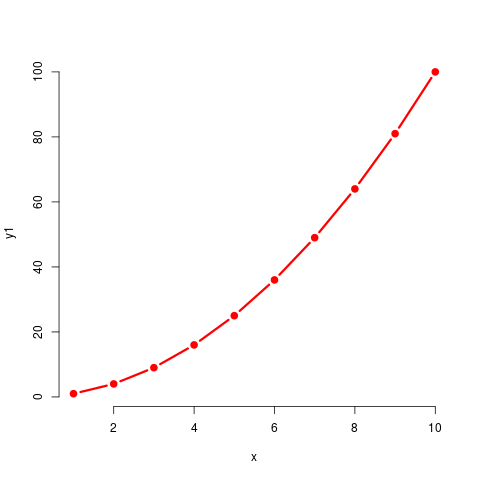
\includegraphics[width=.9\linewidth]{baseplot1.png}
\end{center}
\begin{enumerate}
\item Changing the look of base plot
\label{sec:org2bb0efb}
You have multiple \emph{hidden} arguments you can use to change the look of the plot such as the symbols, whether it plots lines or dots, the color, the font size. Always remember to try the help command. Here is just one example.

\begin{verbatim}
plot(x,y1,type = 'b', frame = F, pch = 19, col = "red" , ylabel = "y", lty = 1, lwd = 3)
\end{verbatim}

How would you include this plot in another document?

\begin{verbatim}
plot(x,y1,type = 'b', frame = F, pch = 19, col = "red" , ylab = "y", lty = 1, lwd = 3)
lines(x,y2, pch = 18, col = "blue", type = "b" , lty = 2, lwd = 1)
lines(x,y3, pch = 17, col = "green" , type = "l", lty=3, lwd = 4)
legend("topleft", legend = c("Line 1", "Line 2", "Line 3"), col = c("red","blue","green"),
       lty = 1:3, cex = 0.8)
\end{verbatim}
\captionof{figure}{\label{orgc21f5a7}
Our base plot with additional data series added.}

\begin{center}
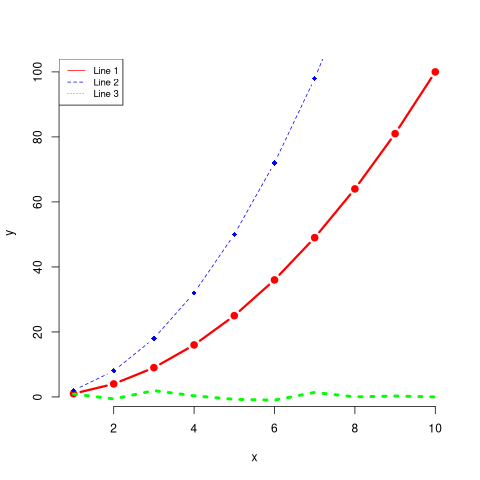
\includegraphics[width=.9\linewidth]{baseplot3.png}
\end{center}
Who wants to try and recreate this in Excel or SPSS?
\end{enumerate}


\item Ggplot
\label{sec:orgb393a9a}
\texttt{ggplot} uses a model where you build things up  bit by bit all in one line, and you can keep adding to the same object. For instance. 

Note that people tend to say "ggplot", but they always mean =ggplot2". Note the number "2". 
\begin{verbatim}
       library(ggplot2)
p  <- ggplot(data = data.frame("x" = x, "y1" = y1, "y2" = y2, "y3" = y3), aes(x = x, y = y1, col= 'r'))
p <- p + geom_point() + geom_line() + theme(legend.position = c(0.2,0.65)) + geom_line(aes(x=x,y=y2, col = "blue")) + geom_line(aes(y=y3,col = "green"))
ggsave("ggplot1.png", width = 8, height = 5, units = "cm") 
\end{verbatim}

\begin{center}
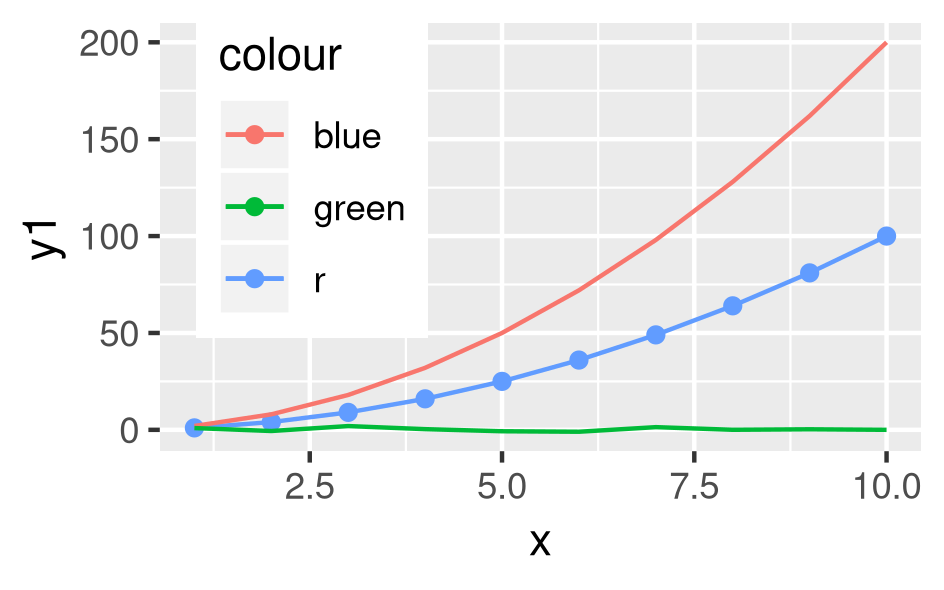
\includegraphics[width=.9\linewidth]{ggplot1.png}
\end{center}

\item Scatter Plots and Box Plots
\label{sec:org6797ce4}
\begin{enumerate}
\item Using the R data set \texttt{mtcars} create in both base plot and ggplot a scatterplot of \textbf{mpg} and \textbf{wt}. What would you expect this to show even before you plot it. Always good to know what you are looking for as a clue to test if something went wrong.
\item Using the R data set \texttt{ToothGrowth} generate boxplots for \texttt{len} and \texttt{dose}. If you are feeling creative overlay the data points on top of the box plot.
\end{enumerate}

\item Lattice
\label{sec:org7f79f0f}
\href{https://stat.ethz.ch/R-manual/R-devel/library/lattice/html/Lattice.html}{Lattice Plot Overview}
\end{enumerate}
\subsubsection{Interaction Plots}
\label{sec:org0728e1a}
What is an interaction plot and when would you like to use one?

I am including this specifically because it was mentioned that is something that is hard to produce in SPSS, and the stats courses thought it could be useful. 
\begin{enumerate}
\item Getting the data
\label{sec:orgad12201}
Download the data from \url{http://personality-project.org/r/datasets/heating.txt}

Okay. It is a text file. Read that into pandas in Python.
\item Pandas Read in Text
\label{sec:orgdd32d63}
\begin{verbatim}
import pandas as pd
url = "http://personality-project.org/r/datasets/heating.txt"
d = pd.read_csv(url, sep = "\t")
d.columns
\end{verbatim}

Did the last line to check if the data imported correctly. 

We want to get plots of degree days versus therms, but we want to do it separately for each type of house to see if there is an \emph{interaction}. That is, is the relationship between degree days and therms different for the different types of houses. Types of houses \emph{interacts} with \texttt{degreedays} when we want to predict \texttt{therms}. 

We will also use some additional python modules to help us make this easier, specifically \texttt{scipy}, \texttt{matplotlib}, and \texttt{statsmodels}. These can be installed via \texttt{pip} (which we used at the beginning of the course). 

\begin{verbatim}
from statsmodels.graphics.factorplots import interaction_plot
from matplotlib import pyplot as plt
fig = interaction_plot(d['degreedays'],d['Location'],d['therms'])
plt.savefig("py-inter-plt.png")
"py-inter-plt.png"
\end{verbatim}

\begin{center}
\includegraphics[width=.9\linewidth]{py-inter-plt.png}
\end{center}

Of course this gives us a "connect" the dots sort of look to our data, because that is what we are doing. Plotting the raw data points. We would prefer to fit a line, a \emph{best} line to our data. We want to pick the line that runs through the data points and is as close as possible. The techniques for doing this, and the theory, come from your stats courses, but we can use those tools here without explanation just to get some practice with the libraries and functions that will later come in handy. 

\begin{verbatim}
from statsmodels.formula.api import ols
ols_d = ols(formula = "therms ~ degreedays * Location",data = d)
myfits = ols_d.fit()
plt.clf()
f = plt.figure()
a = f.gca()
interaction_plot(d['degreedays'],d['Location'],myfits.fittedvalues,plottype="line",ax = a)
a.legend = None
interaction_plot(d['degreedays'],d['Location'],d['therms'],plottype='scatter',ax = a)
plt.savefig("py-inter-fit-plt.png")
"py-inter-fit-plt.png"
\end{verbatim}

\begin{center}
\includegraphics[width=.9\linewidth]{py-inter-fit-plt.png}
\end{center}
\end{enumerate}
\subsection{Session 8 Programming Experiments}
\label{sec:org4ae2a0b}
\subsubsection{Experimental Programming in Python}
\label{sec:orgf41d4ae}
The components of a typical experimental program in psychology involve some combination of showing something on a computer and getting a response from the participant. This typically means you will need some way of talking to the graphics part of the computer (to place text or images on the monitor), and some way of listening to the computer to record keyboard, button box, or mouse presses. \emph{Listening} for eye movements or EEG is an extension of this basic approach. 

It is possible (and sometimes more direct) to use python library that more directly address these goals, such as \href{http://pyopengl.sourceforge.net/}{pyopengl} for graphics or \href{https://www.pygame.org/news}{pygame} for getting joystick input, but in general never reinvent the wheel if you don't have to. As computer are common tools of psychological research there have been some excellent libraries that serve as one-stop shops for our needs. The one we will use in this course is \href{https://www.psychopy.org/}{psychopy}.
\begin{enumerate}
\item Psychopy Library
\label{sec:orga46f5e2}
\begin{enumerate}
\item For future reference you should note that psychopy is building in increasing support for performing online studies. These extension often rely on another language, javascript. We will \textbf{not} be using these extension here, but if you master the basics you will be able to extend your use on your onw.
\item Resources for Psychopy.
\begin{enumerate}
\item The authors of the Psychopy library have written an entire \href{https://us.sagepub.com/en-us/nam/building-experiments-in-psychopy/book253480\#contents}{textbook} on using python for psychology experiments that includes the online extensions. That is a good resource to pursue things after this course.
\item On the psychopy website is an \href{https://www.psychopy.org/coder/coder.html}{introduction} to using the coder component of psychopy.
\item Searching online with \texttt{psychopy tutorial} will get you a variety of hits. Note that you want to emphasize the \texttt{coder} version. Maybe the \texttt{builder} will meet your needs, but better to start with the \texttt{coder} version and use the \texttt{builder} for efficiency. In many cases it will be harder to build a complex experiment in the \texttt{builder} than by directly using the \texttt{coder} version.
\end{enumerate}
\end{enumerate}
\begin{enumerate}
\item Psychopy Demos
\label{sec:org3559cca}
Purpose: Demonstrate that you have psychopy installed and functioning

Navigate to where installed. Look in (via terminal) \texttt{cd \textasciitilde{}/.lib/python3.6/site-packages/psychopy/demos/coder/stimuli/}

\texttt{python3 face\_jpg.py}

Run a few other demos.

Save one of the demos with a slightly altered name (so you don't overwrite the original). Open it up in your editor and change one tiny thing. Maybe the color of something or the size. Save it. Close. And then run your altered demo. 
\item Psychopy Exercise
\label{sec:org1fef509}
This demo still needs testing
\begin{enumerate}
\item Open up a terminal.
\item Begin a python session
\item \texttt{from psychopy import visual,core}
\item Create a window
\texttt{mywin = visual.Window(size = (640,480))}
\item Test it
\texttt{mywin.flip()}
\item Why is it called \emph{flip}?
\item Add a red rectangle.
\texttt{myrect = visual.Rect(mywin, linewidth = 0, fillcolor = "red", size = [.2,.2],pos=[0,0],units="norm")}
\item Draw it
\texttt{myrect.draw()}
\item Show it
\texttt{mywin.flip()}
\item Clean up and shut down in an orderly way
\texttt{core.quit()}
\end{enumerate}
\item Extensions
\label{sec:org3869839}
To work on these examples you will want to consult the \href{https://www.psychopy.org/api/api.html}{psychopy API} to see what functions do what, and what the arguments are that you need to supply. 
\begin{enumerate}
\item Change the color of the square.
\item Move the Square.
\item Add some text
\item Keep the window open for a certain amount of time, and then close it when that time has elapsed.
\item Run any of the demo programs you can find in the \texttt{.../psychopy/demo/coder/stimuli/} directory.
\item Change something in the demo you are running and see what the effect is.
Note you may want to save the original file with a new name and hack on the one with a new name. That way it will be easier to go back to the original if you break something.
\end{enumerate}
\item Simple Tutorials
\label{sec:orgac3a93e}
\href{https://www.psychopy.org/coder/tutorial1.html}{Here} is the first Psychopy tutorial 

See if you can get this to work. 

Another idea: \href{https://www.psychopy.org/coder/tutorial2.html}{A formula for JND}
\end{enumerate}

\item Homework (can start in class)
\label{sec:org55d365c}
\begin{enumerate}
\item Provide me with a name of the basic variety or example of the experiment you intend to code (with at least one reference using that task).
\item Provide a written (not code) outline of what you will need to do to implement the task.
\item Provide links to any existing versions of the task that you hope to be able to adapt for your usage.
\item \emph{Be very basic.} Simple recall. Simple reaction time. Stroop. Picture versus word memory. The goal is to get something minimal working to prove "proof-of-concept"; not to actually have a reliable experiment coded.
\end{enumerate}
\end{enumerate}
\subsection{Session 9 Report Writing}
\label{sec:orgfb86d61}
\subsubsection{Writing a simple report}
\label{sec:org6f0e3f2}
\begin{enumerate}
\item We will use emacs. Open it up.
\item We will use R.
In the future, you might prefer to use the \texttt{knitr} package. But I am sticking with this \emph{org-babel} so that I have one less new thing to introduce. However, it is an amazing \href{https://yihui.name/knitr/}{package}, that you may want to learn more about.
\item Testing
\begin{itemize}
\item If you have emacs correctly installed and a working latex installation than you should be able to open \texttt{testLatex.org} in emacs and type \texttt{C-c C-e l p} and you will see a new pdf file in your directory that you can open up (also in emacs).
\item If you have R and ESS installed properly you can open up \texttt{testRBabel.org} in emacs and type \texttt{C-c C-e l p} and you will see a new pdf appear that has the code and graphic that you just processed.
\end{itemize}
\end{enumerate}
\subsubsection{Mixing Code and Text for reproducibility}
\label{sec:orga6ae414}
\begin{enumerate}
\item Intro
\label{sec:org94a4dda}
Org-mode in emacs is a version of a markdown language (other markdowns are github flavored markdown and R markdown). They all have the same basic goal of letting you type simple text and have something else behind the scenes necessary for producing a webpage or a pdf file. In addition, org-mode has a component \emph{bable} component that can also read and execute code putting pretty, formatted output into your final document. This week we will experiment with this capability.
\item Getting started with Orgmode
\label{sec:orge28b065}
\begin{enumerate}
\item Open emacs. Do you know what directory you are in? Try \texttt{M-x pwd} and look at the minibuffer. What does the "M" stand for in that command. What key does it mean?
\item Open a file and give it a name. Make the extension \texttt{.org}.
\item Type an asterisk (*) followed by a space and a name for your first header.
Ask me about shortcut keys if you want to work faster.
\item Save
\item \texttt{C-c C-e t A} You should see the output in a new buffer. Do the \texttt{C-c C-e} part again and look at all the different output options available.
\end{enumerate}
\item Getting help
\label{sec:org660aac8}
Emacs (and orgmode) have good help. \texttt{C-h i}. H is for help and i is for information. You could also use f for function or k for key. 
\item Practice
\label{sec:org95c4d26}
\begin{enumerate}
\item Write some text that includes a bold word and an italics word.
Collaborate to figure out how to do this.
\item Make a list with numbers and reorder things.
\item Add a link to any website you want.
\item Export as a web page and open up the file in firefox and show that your link works.
\item Add a link to an image.
\item Export the same basic file as a pdf. Verify the link works there too. Make sure you can see the picture.
\end{enumerate}
\item Source code
\label{sec:org225bc38}
It is possible to put computer code in files and have it executed at the time the document is compiled. Of course this is not a program in the conventional sense. You will not be getting user input. What it is is a way for you to document fully what analyses were done and how they were done so that others can repeat fully your analysis. It allows you an easy way to update work when new files come in or as other changes to work appears. You will never again search for a missing image file when the images are made at the time the file is compiled.

There are "cookbooks" with numerous examples \footnote{\url{http://ehneilsen.net/notebook/orgExamples/org-examples.html\#sec-22-1}}. 
\begin{enumerate}
\item Reproducible Research/Literate Coding
\label{sec:org44f77d6}
These are two different, but mutually reinforcing concepts. \href{https://en.wikipedia.org/wiki/Literate\_programming}{Literate coding} is writing code where the emphasis is on embedding the pure code in a textual environment intended to have a human reader. The computer doesn't need the code explained by human users do, so right the code for them with ample explanations. By doing so, you make it easier for others to \href{https://www.pnas.org/content/112/6/1645/}{reproduce} your work, and to make suggestions to improve it. 
\item Testing the inclusion of source code
\label{sec:org58d3884}
Open up the test file for babel and verify that you can get it to compile to pdf. Then change or add something. Since you already submitted some R content, you should be able to find some code you know works to test with. 
\item Can you combine source code from multiple languages?
\label{sec:org0f81799}
That depends on the tool. Rstudio is developed around R, but with org-babel you can combine multiple languages in one document. Add a src block for python and show that it too can be type set and output generated for a pdf. 
\item Tables.
\label{sec:org1805884}

Pretty much happens automatically. You may have to play with the \emph{header} arguments to get exactly the look you want. The \emph{header} arguments are those things appearing on the \texttt{+\#Begin\_Src} line. 

\begin{verbatim}
d <- data.frame(foo=c('a','b','n'), bar=c(1.0/3.0,22,32))
d
\end{verbatim}

\begin{center}
\begin{tabular}{lr}
foo & bar\\
\hline
a & 0.333333333333333\\
b & 22\\
n & 32\\
\end{tabular}
\end{center}

\item What is an inline result?
\label{sec:org32d3276}
An inline result is one that appears at the correct place in the text. 

The mean of 100 mean 0 normally distributed numbers is -0.0425027071235594.

\item Can I include references?
\label{sec:org587ef33}
Yes. Of course you can. 

\begin{enumerate}
\item Using bibtex
\label{sec:org0381965}
There are other, better, approaches (e.g. biblatex), but we will start with the bare bones method for demonstrating the basic capabilities.

Open up the test bib file and make sure you have the .bib file. Make sure they are both stored in the same directory and that you open the .org file in emacs. Then, if you have the right packages for latex installed, you should be able to \texttt{C-c C-e l l} to produce a file ending with .tex as an extension. Open this in emacs and then keep doing \texttt{C-c C-c} while reading the minibuffer and doing it until it tells you to stop. Then you should have a pdf with a correctly placed citation. 


\item Practice
\label{sec:org4cc3a75}
Go to \url{https://scholar.google.ca} and set your preferences to show the export as bibtex link. Then grab any reference and add it to the .bib file. Then add a citation to the test file and recompile. Show that you can get the second reference to work.
\end{enumerate}
\end{enumerate}
\end{enumerate}


\subsubsection{Homework}
\label{sec:org0e31db9}
Submitting a small .org file and .bib file that will compile correctly to a final pdf and that includes at least one source code block, one reference, one link, one plot, one inline usage, and a bibilography with at least one reference. 
\subsection{Session 10 Coding the Experiment}
\label{sec:orge8ee1a9}
These last three sessions are generally open with the idea that students will 
\begin{enumerate}
\item Code up an experiment in Psychopy (e.g. stroop or reaction time or simple associative memory task).
\item They will collect data on their classmates
\item They will write up a report on their experience that includes the source code and simple data analyses.
\item They will include some references to pertinent literature.
\item They will do this using a reproducible mechanism providing both the raw file and the processed file (pdf preferred, html acceptable.
\end{enumerate}
\subsection{Session 11 Collecting the Data}
\label{sec:org302bc12}
Data collection.
\subsection{Session 12 Presentations}
\label{sec:orgee8eb69}
Presentation. Should be able to produce an html 5 slide show of some of the motivation/method/data with graphics.

Can also work on final report and technical questions. The final report will have a later due date. 
\begin{itemize}
\item Other
\end{itemize}
\subsection{Instructions for Burning Xubuntu to USB}
\label{sec:orgc5688be}
The following instructions were cultivated from the following three webpages and represent a blend of their techniques:
\begin{itemize}
\item \url{https://forums.linuxmint.com/viewtopic.php?f=42\&t=287353\#p1590473}
\item \url{https://www.dionysopoulos.me/portable-ubuntu-on-usb-hdd/}
\item \url{https://superuser.com/questions/376470/how-to-reinstall-grub2-efi}
\end{itemize}

The first one is the most comprehensive, but there are useful ideas in both of the others. One thing to note is that if you are using a \emph{BIOS} computer (that is a computer that is still booting with a true BIOS), then you can just use the Xubuntu USB without special fiddling. The only special things you need to do are to make sure you pick the usb for both the location for installing the OS \textbf{and} the location for the boot program. 

However, if you are using a UEFI system (and most of us are at this point) then a bug in the Ubuntu installation disk (which seems to have been around for ages) will not install the boot program to the USB you indicated, but rather will install it on to your home directory. That can make life difficult for all, and scary for the novice. 

I tried pretty much all the routines in the linux mint description, and not all of them worked reliably for me. They would usually work on the computer I used to generate them, but not on random other computers I tried to boot from. For that reason, I went with this hybrid method that seemed reliable for UEFI systems.

\subsubsection{Installation Instructions for Installing Xubuntu (and probably other -buntus) to a USB from a USB.}
\label{sec:org1aa4178}
\begin{enumerate}
\item You need at least two usbs to be able to be plugged in.
\item Boot the live Xubuntu disk. To do this you will first have to figure out what special magic is needed to make your computer allow usb booting. Each manufacturer and OS system has their own combination of keys and boot start-up settings that are required. You have to figure that out first, before starting here.
\item Make sure to open up the power management settings and make sure nothing turns off or goes to sleep while you are doing this. Pay attention to the \texttt{Display} tab. Even on power this will put your screen to sleep, which can cause you to lose all your work. Set them to "never" by dragging all the way to the left of the sliders.
\item After the live USB is booted (you selected Try Ubuntu) open a terminal and launch \texttt{gparted}. Gparted is a program for partitioning drives.
\item Make sure the device selected on gparted is the USB you want to install the system to. You can use the size to help. The usb you  booted from will probably have type ISO 9600. If in doubt, plug in the new USB after starting gparted and noting all the devices, and then refresh devices and see which one is the new one.
\item Make a new \texttt{GPT} partition table for the USB. This will wipe out all the data you have on that USB (or any other disc you incorrectly set).
\item Make a 200 MB FAT32 partition.
\item Make the rest EXT4 for simplicity.
\item Apply those partitions so that you can \ldots{}
\item Set the \texttt{efi} and \texttt{boot} flags for the 200 MB FAT32 parition. Use the manage flags menu.
\item Right click on that partition and click on the info tab. Write down the UUID. It will probably be two four digit numbers separated by a hyphen.
\item Close gparted.
\item Back in your terminal, run \texttt{ubiquity -b}. This will start the installation program, but will not require you to install a boot loader. You will do this manually later.
\item Follow the screens until you get to where to install things. You want \texttt{something else}.
\item Chose the EXT4 partition of the USB you formatted for change. Select it as an EXT4 and mount to "root" which is \texttt{/}. Do not format (you already did that).
\item Install the system.
\item When it is done continue with "continue testing."
\item For the rest of this I am assuming that your USB is /dev/sda and your FAT32 partition is /dev/sda1. You need to replace those names with the correct names of your partition for you system. If in doubt, open up gparted again to verify what it is.
\item Log on to your wifi and make sure you have network connectivity. Ethernet is fine to if you have been using that.
\item Open up your terminal. And enter the following commands:
\begin{verbatim}
sudo mount /dev/sda2 /mnt
mkdir /mnt/boot/efi
sudo mount /dev/sda1 /mnt/boot/efi
nano /mnt/etc/fstab
\end{verbatim}
What you are doing here is "mounting" your USB at a particular mount point on the booted live system. You will now be able to see those partitions and write to them. First, you mount the root at the top, and then you boot your boot system in its proper place in the hierarchy. You may or may not need to create the directories. 

The editing of \texttt{fstab} is to make sure that your system knows the correct location for booting in the future. By using a universal identifier your system should update properly.
\item Edit the fstab to point to your usb's boot location thus:
In the file \texttt{fstab} comment out (with a \emph{\#}) any line for boot/efi and replace the UUID part with the UUID you wrote down earlier making a new line. This way you keep the old one to refer to if necessary while making a new one.
Your new one should look something like: \texttt{UUID=0123-ABCD /boot/efi vfat defaults 0 1}
\item Then you exit out of nano and resume in your terminal.
\begin{verbatim}
for i in /dev /dev/pts /proc /sys; do sudo mount -B $i /mnt/$i; done
sudo cp /etc/resolv.conf /mnt/etc/
modprobe efivars
sudo chroot /mnt
\end{verbatim}

What you are doing here is giving your new usb access to functionings of the current running system that it will need later when we trick it into thinking that it is the root.
\item Now we install the program we will use for booting \texttt{grub2}. We will do this from a \emph{chroot} environment. Where we \textbf{ch} ange the \textbf{root} so that we can put grub on /dev/sda and not on our hard disk
\item \textasciitilde{}apt install grub-efi \textasciitilde{}
\item If that did not work you may have to \texttt{apt update} first to populate your list of software
\item \textasciitilde{}grub-install -d \emph{usr/lib/grub/x86\(_{\text{64}}\)-efi --efi-directory=/boot/efi} --removable /dev/sda
\item The removable bit is to help with the proper updating
\item It may not be necessary to do a \texttt{update-grub} at this point, but I was getting fatigued and did not thoroughly check. I just did one, and it seemed to work.
\item Need to exit chroot and then umount all the mounted directories. You do this by \texttt{umount} in order all the things you \texttt{mount} ed before and in the opposite order. Especially your /mnt/boot/efi which you do not want to corrupt after all this.
\item Then you should be able to boot your system on a uefi computer
\end{enumerate}
\subsection{Interesting Programs}
\label{sec:org0f946a4}
As part of their exercises, students locate an interesting program from the Xubuntu software collection. This is a list of the different programs students found and reported on.
\subsubsection{Programs}
\label{sec:orgec3ce1e}
\begin{enumerate}
\item Android Studio
\label{sec:org9cfe45a}
\begin{enumerate}
\item Program Description
\label{sec:orge68a0b9}
Android Studio is an IDE (Integrated Development Environment) for building your own Android apps.
It automatically creates the file structure for a number of useful basic App templates, has a useful GUI, and supports virtualization of a number of android devices (for example, simulating a Google Pixel3 XL).
\item Review
\label{sec:orgb85344e}
I'm just getting started with it and the Kotlin language it uses, but so far it is great. My plan for this is to build an app that encompasses a number of basic phone functions while excluding distracting factors like social media, email, etc.
\end{enumerate}
\item Caprine
\label{sec:orga7ee711}
\begin{enumerate}
\item Program Description
\label{sec:org41def90}
Caprine is an unofficial Facebook Messenger app for linux.
\item Review
\label{sec:org200b71d}
I like Caprine because I use Facebook Messenger very often on my Windows/MacOS desktop.

Despite being an unofficial app, Caprine looks, feels, and performs perfectly like the official Windows/MacOS desktop app.

Functions almost identically to how it does on Windows. It looks like the Ubuntu compatible version was actually created by Discord themselves and not by a third party developer. I would definetely recommend it to others as I feel it's vastly superior to Skype (which is honestly only used in highly professional settings these days). Can run small communities (clubs, class discussions, etc.) and can be used for collaboration in all sorts of formats. I chose it because it is something I personally use frequently to keep in touch with friends (especially helpful for very large groups).

I like Caprine because I use Facebook Messenger very often on my Windows/MacOS desktop.

Despite being an unofficial app, Caprine looks, feels, and performs perfectly like the official Windows/MacOS desktop app.
\end{enumerate}
\item Amoebax
\label{sec:orgcfb43cc}
\begin{enumerate}
\item Program Description
\label{sec:orga588d1d}
This is a game similar to tetris.

A program that was originally developed for the purposes of playing games online with friends, Discord is now used as an alternative to Skype, primarily due to its multi-purpose functionality. It allows for easy collaboration through screensharing, voice, text and video-chat and is entirely free. It can be used as a social hub as well as it runs continually and can be moderated, and is not a singular call.
\item Review
\label{sec:org8d4f72a}
I downloaded this game because I thought it would be a fun and interesting one. After playing this game, it seems like it's very similar to Tetris, but uses different characters. I would recommend this game to those who like Tetris.  

Functions almost identically to how it does on Windows. It looks like the Ubuntu compatible version was actually created by Discord themselves and not by a third party developer. I would definetely recommend it to others as I feel it's vastly superior to Skype (which is honestly only used in highly professional settings these days). Can run small communities (clubs, class discussions, etc.) and can be used for collaboration in all sorts of formats. I chose it because it is something I personally use frequently to keep in touch with friends (especially helpful for very large groups).
\end{enumerate}
\item GIMP
\label{sec:orgf7bf1cd}
\begin{enumerate}
\item Program Description
\label{sec:org5fddf61}
GIMP is a photo editing software similar to photoshop.
\item Review
\label{sec:org8b1dcf0}
I like GIMP because I want to learn photo editing skills and Photoshop is too expensive.
\end{enumerate}
\item Bastard Tetris
\label{sec:org878d51d}
\begin{enumerate}
\item Program Description
\label{sec:org6543441}
This is a small game
\item Review
\label{sec:org264b84a}
I liked it
\end{enumerate}
\item Discord
\label{sec:org531013d}
\begin{enumerate}
\item Program Description
\label{sec:org1ca976a}
A program that was originally developed for the purposes of playing games online with friends, Discord is now used as an alternative to Skype, primarily due to its multi-purpose functionality. It allows for easy collaboration through screensharing, voice, text and video-chat and is entirely free. It can be used as a social hub as well as it runs continually and can be moderated, and is not a singular call.
\item Review
\label{sec:org19ff716}
Functions almost identically to how it does on Windows. It looks like the Ubuntu compatible version was actually created by Discord themselves and not by a third party developer. I would definetely recommend it to others as I feel it's vastly superior to Skype (which is honestly only used in highly professional settings these days). Can run small communities (clubs, class discussions, etc.) and can be used for collaboration in all sorts of formats. I chose it because it is something I personally use frequently to keep in touch with friends (especially helpful for very large groups).
\end{enumerate}
\item Snake4
\label{sec:orgcc19d18}
\begin{enumerate}
\item Description:
\label{sec:org440b0be}
Snake4 is a basic video game where the player controls a line resembling a snake which is constantly moving and grows in length as it collects food. The main goal is to make the snake as large as possible and the game will be over once you reach the maximum limit. Snake4 is a classic game that is entertaining and relatively easy to play. I downloaded this program so that I can distract myself if Xubuntu gives me less needed anxiety and distress. Stricly not to be used in lectures.
\item Review:
\label{sec:org10278cd}
Snake4 is a nostalgic game which many of us has encountered as our default game application before the smart phone era. The application provided a simple, quick and enjoyable leisure time activity. I still enjoy this program because it reminds me of the simplier times. If you also want to feel a little bit of nostalgia I definetly recommend downloading this entertaining game.
\end{enumerate}
\item Polar
\label{sec:org9347b26}
\begin{enumerate}
\item Short Description
\label{sec:orgd9c7087}
      Polar is a package for organizing and tracking documents, including \^{}M
pdfs and webpages. You can tag, highlight and share your documents.
\item Review
\label{sec:org22267e8}
      I think Polar can be helpful for literature reviews, when you need to \^{}M
keep track of lots of online and downloaded articles.
\end{enumerate}
\item Gparted and Disks\ldots{}
\label{sec:orgaf7d548}
\begin{enumerate}
\item Description
\label{sec:orgb377ab4}
Gparted is a package for formatting USB drives. Disks allows them to be mounted.
\item Review
\label{sec:orgbe99df9}
These packages came in handy for reformatting the USB drives when it became necessary. Either due to my experimenting gone wrong, or when they needed to be formatted as fat32 and partitioned so that Xubuntu could be installed on them.
\end{enumerate}
\item Chromium
\label{sec:org00b53a2}
\begin{enumerate}
\item Program Description
\label{sec:org3b8507d}
Chromium is a web browser that is the counterpart of Google Chrome on Linux system.
\item Review
\label{sec:org6b6d7c1}
Chromium is pretty much identical to Chrome. You can log in to your google account and manage bookmarks, histories, and settings. Optional extension programs within the browser are compatible to the environment as well.
\end{enumerate}
\item Tasque
\label{sec:orgd0d8ce1}
\begin{enumerate}
\item Description:
\label{sec:orgadf80c1}
An application that creates and organizes to-do lists 
\item Review:
\label{sec:orgc8278b2}
It is an average reminders application that has the standard features such as adding additional notes to reminders, the ability to categorize them, etc. Overall, I would stick to your standard phone reminders application due to the ease of accessing it.
\end{enumerate}
\item Bovo Review
\label{sec:org3ef029d}
I liked it because it looked nice and simple to play. 

I also made sure it was small in its size that does not take up 4GB to save in my usb.
\item gbrain
\label{sec:org2351417}
\begin{enumerate}
\item Description
\label{sec:org6272335}
A game that helps you train your brain
\item Review
\label{sec:org19d51c1}
I like this game as it is challenging to all ages
\end{enumerate}
\end{enumerate}

\section{Improvements:}
\label{sec:orgb7ce5a8}
I recommend starting the course with R rather than python because it is more useful for those getting a psychology degree (I think) as it is more specific to data analysis. I liked how we were introduced to both R and python in this course. 
\end{document}
